
\section{Manual de usuario}

La aplicación entregada se compone en realidad de cinco partes:

\begin{itemize}
 \item SWAML
 \item configWizard
 \item FOAF Enricher
 \item KML Exporter
 \item Buxon
\end{itemize}

Cada uno de estas partes toman la forma de un script Python que puede ser 
invocado mediante su intérprete. La ayuda de cada uno de ello se encuentra
disponible llamandolo con la opción \texttt{--help}, aunque se pasará a 
explicar con más detalle el uso de cada una de estas cinco aplicaciones.

\subsection*{SWAML}

Es la aplicación principal, la que desarrolla el propósito principal del
proyecto. Su funcionalidad se provee por medio del script \texttt{swaml.py}.
Su uso es bien sencillo: como se puede ver en la captura de la 
figura~\ref{fig:swaml} se le invoca acompañado de un único parámetro obligatorio 
que indica la ruta donde esta la configuración que se le quiere pasar a 
SWAML. Inmediatamente se desemboca todo el proceso sin interacción
alguna con el usuario más que las estadísticas informativas que se 
imprimen al final de cada fase importante del proceso. Si no se
imprime ningún error el proceso habrá concluido satisfactoriamente.

\begin{figure}[H]
	\centering
	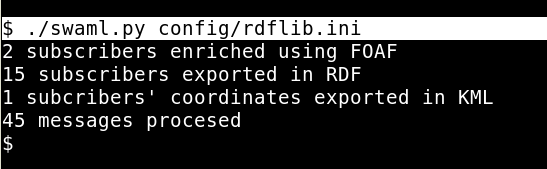
\includegraphics[width=10cm]{images/screenshots/swaml.png}
	\caption{SWAML}
	\label{fig:swaml}
\end{figure}

\subsection*{configWizard}

Por medio del script \texttt{congWizard.py} se provee un asistente para
ayudar al usario a crear ficheros de configuración según el formato
que debe recibir SWAML. Tal y como se puede ver en la captura de pantalla
de la figura~\ref{fig:configWizard} el script recibe la ruta destino del 
fichero donde se quiera guardar la configuración. El proceso es sencillo: 
el asistente va pidiendo una serie de parámetros al usuario, ofreciendole
un valor por defecto, hasta que haya recopilado toda la información necesaria,
volcándolos inmediatamente a disco con el formato adecuado en la ruta 
indicada por el usuario.

\begin{figure}[H]
	\centering
	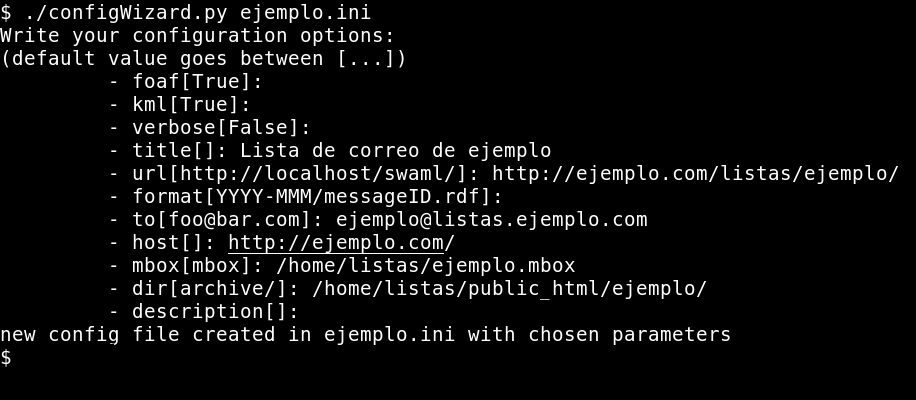
\includegraphics[width=14cm]{images/screenshots/configWizard.png}
	\caption{configWizard}
	\label{fig:configWizard}
\end{figure}

Un fichero de ejemplo (que se acompaña con la aplicación) podría ser el
siguiente:

\begin{figure}[H]
\begin{lstlisting}
[SWAML]
title = Example mail list
description = Example description
host = http://example.com/
dir = /var/www/lists/archives/example/
url = http://example.com/lists/archives/example/
mbox = /var/lib/mailman/archives/public/example.mbox
format = YYYY-MMM/postID.rdf
to = example@lists.example.com
kml = yes
foaf = yes
\end{lstlisting}
\caption{Ejemplo de fichero de configuración}
\label{fig:ejemplo-config}
\end{figure}

\subsection*{FOAF Enricher}

Aunque esta funcionalidad se provee en el core de la aplicación principal,
en determinados casos puede ser necesario su uso de manera independiente.
Así el script \texttt{foaf.py} recibe la ruta de un fichero RDF con los
suscriptores de una lista de correo, busca el fichero FOAF de cada uno y
lo enriquece con determinadas propiedades (el propio URI del FOAF, fotografía,
coordenadas geográficas, etc).

\begin{figure}[H]
	\centering
	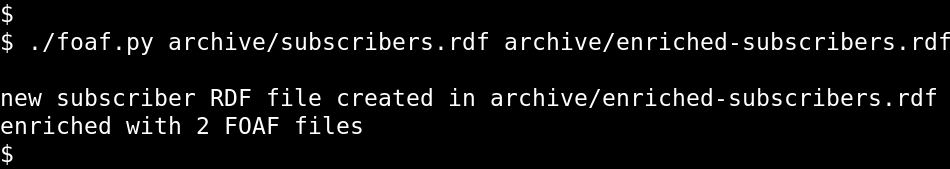
\includegraphics[width=12cm]{images/screenshots/foaf-enricher.png}
	\caption{FOAF Enricher}
	\label{fig:foaf-enricher}
\end{figure}

\subsection*{KML Exporter}

Al igual que en el caso anterior, la funcionalidad dada por este componente
de manera independiente forma también parte de la aplicación principal. En ese
caso el script \texttt{kml.py} toma como primer parámetro la ruta de un fichero
de suscriptores enriquecido con información geográfica y genera otro fichero
en formato KML posicionando geográficamente los suscriptores.

\begin{figure}[H]
	\centering
	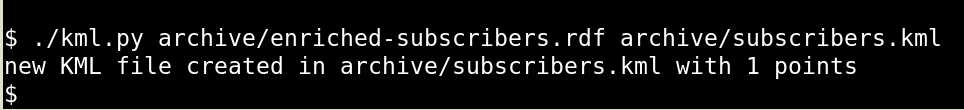
\includegraphics[width=12cm]{images/screenshots/kml-exporter.png}
	\caption{KML Exporter}
	\label{fig:kml-exporter}
\end{figure}

Una manera inmediata para aprovechar esta exportación es utilizar Google Maps para visualizar esos
puntos\footnote{\url{http://maps.google.com/maps?q=http://swaml.berlios.de/demo/subscribers.kml}},
como se puede ver en la figura~\ref{fig:googlemaps}.

\begin{figure}[H]
	\centering
	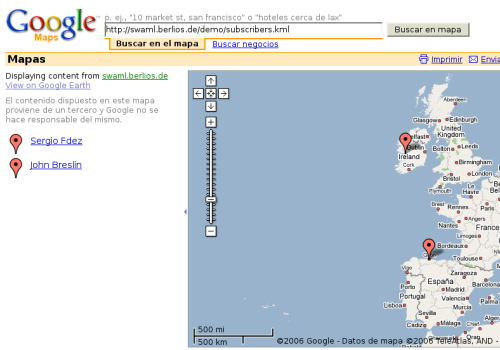
\includegraphics[width=10cm]{images/screenshots/googlemaps.png}
	\caption{Google Maps}
	\label{fig:googlemaps}
\end{figure}

\subsection*{Buxon}

Buxon es un visor de foros exportados con el vocabulario SIOC. Básicamente 
recibe la URI de un \texttt{sioc:Forum} y recompone en forma de árbol los
hilos de conversación definidos. En la figura~\ref{fig:buxon} se puede ver
una captura de la aplicación en acción, que tiene un buscador parecido con 
los navegadores Web convencionales.

\begin{figure}[H]
	\centering
	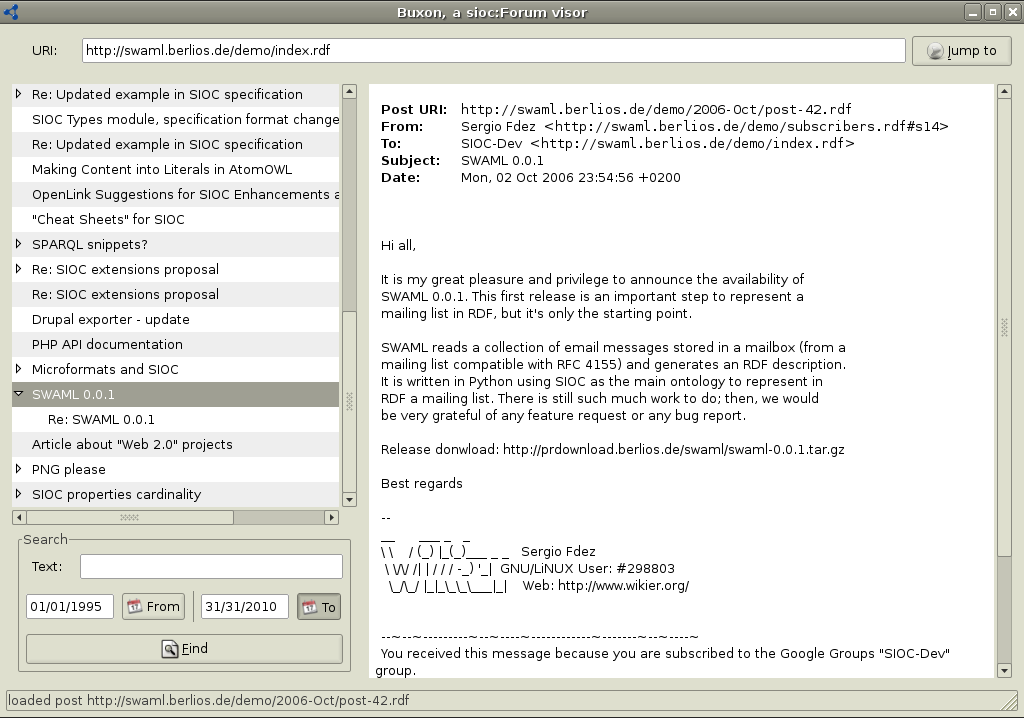
\includegraphics[width=16cm]{images/screenshots/buxon.png}
	\caption{Buxon}
	\label{fig:buxon}
\end{figure}

Su uso es bastante sencillo: sólo necesita recibir, bien como parámetro en linea
o en la barra de direcciones habilitada, la URI de un \texttt{sioc:Forum}.
Haciendo click en el boton \textit{"ir a"} la aplicación analizará esa URI y reconpondrá
todos los mensajes que contenga, listándolos en forma de conversación como si se estuviera
viendo con un cliente de correo tradicional. Además el usuario podrá hacer búsquedas
sencillas por contenido y por rango de fechas.
